\documentclass[a4paper,12pt]{article} % тип документа

% Поля страниц
\usepackage[left=2.5cm,right=2.5cm,
    top=2cm,bottom=2cm,bindingoffset=0cm]{geometry}
    
%Пакет дял таблиц   
\usepackage{multirow} 
    
%Отступ после заголовка    
\usepackage{indentfirst}


% Рисунки
\usepackage{floatrow,graphicx,calc}
\usepackage{wrapfig}

% Создаёем новый разделитель
\DeclareFloatSeparators{mysep}{\hspace{1cm}}

% Ссылки?
\usepackage{hyperref}
\usepackage[rgb]{xcolor}
\hypersetup{				% Гиперссылки
    colorlinks=true,       	% false: ссылки в рамках
	urlcolor=blue          % на URL
}


%  Русский язык
\usepackage[T2A]{fontenc}			% кодировка
\usepackage[utf8]{inputenc}			% кодировка исходного текста
\usepackage[english,russian]{babel}	% локализация и переносы


% Математика
\usepackage{amsmath,amsfonts,amssymb,amsthm,mathtools, mathrsfs}


% Что-то 
\usepackage{wasysym}


\begin{document}
\begin{center}
	\footnotesize{ФЕДЕРАЛЬНОЕ ГОСУДАРСТВЕННОЕ АВТОНОМНОЕ ОБРАЗОВАТЕЛЬНОЕ 			УЧРЕЖДЕНИЕ ВЫСШЕГО ОБРАЗОВАНИЯ}\\
	\footnotesize{МОСКОВСКИЙ ФИЗИКО-ТЕХНИЧЕСКИЙ ИНСТИТУТ\\(НАЦИОНАЛЬНЫЙ 			ИССЛЕДОВАТЕЛЬСКИЙ УНИВЕРСИТЕТ)}\\
	\footnotesize{ФАКУЛЬТЕТ ОБЩЕЙ И ПРИКЛАДНОЙ ФИЗИКИ\\}
	\hfill \break
	\hfill\break
	\hfill\break
	\hfill \break
	\hfill \break
	\hfill \break
	\hfill \break
	\hfill \break
	\hfill \break
	\hfill \break
	\hfill \break
	\hfill \break
	\hfill \break
	\hfill \break
	\large{Лабораторная работа № 3.3.4\\\textbf{Эффект Холла в полупроводниках}}\\
	\hfill \break
	\hfill \break
	\hfill \break
	\begin{flushright}
		Серебренников Даниил\\
		Группа Б02-826
	\end{flushright}
	\hfill \break
	\hfill \break
	\hfill \break
	\hfill \break
	\hfill \break
\end{center}
\hfill \break
\hfill \break
\hfill \break
\hfill \break
\hfill \break
\hfill \break
\begin{center}
	Долгопрудный, 2019 г.
\end{center}
\thispagestyle{empty}
\newpage

\textbf{Цель работы:} измерение подвижности и концентрации носителей заряда в полупроводниках.

\textbf{В работе используются:} электромагнит с источником питания, миллиамперметр, милливебметр, реостат, цифровой вольтметр, источник питания, образец легированного германия.


\section{Рассчетные формулы}
	Эффект Холла - явление возникновения поперечной разности потенциалов при помещении проводника с постоянным током в магнитное поле.
	\begin{itemize}
		\item
			ЭДС Холла:
			\begin{equation}
				\label{E}
				\mathscr{E_\text{х}} = U_{34} - U_0;
			\end{equation}
		\item
			Постоянная Холла:
			\begin{equation}
				\label{R}
				R_\text{х} = -\frac{\mathscr{E_\text{х}}}{B} \cdot \frac{a}{I};
			\end{equation}
		\item
			Концентрация носителей тока в образце:
			\begin{equation}
				\label{n}
				n = \frac{1}{R_\text{х} e}
			\end{equation}
		\item
			Удельная проводимость материала образца:
			\begin{equation}
				\label{sigma}
				\sigma = \frac{I L_{35}}{U_{35}al}
			\end{equation}
		\item
			Подвижность носителей тока:
			\begin{equation}
				\label{b}
				b = \frac{\sigma}{en}
			\end{equation}
		
	\end{itemize}
\section{Экспериментальная установка}
	Электрическая установка для измерения ЭДС Холла представлена на~(\ref{ris:ustanovka}).
	\begin{figure}[H]
		\center{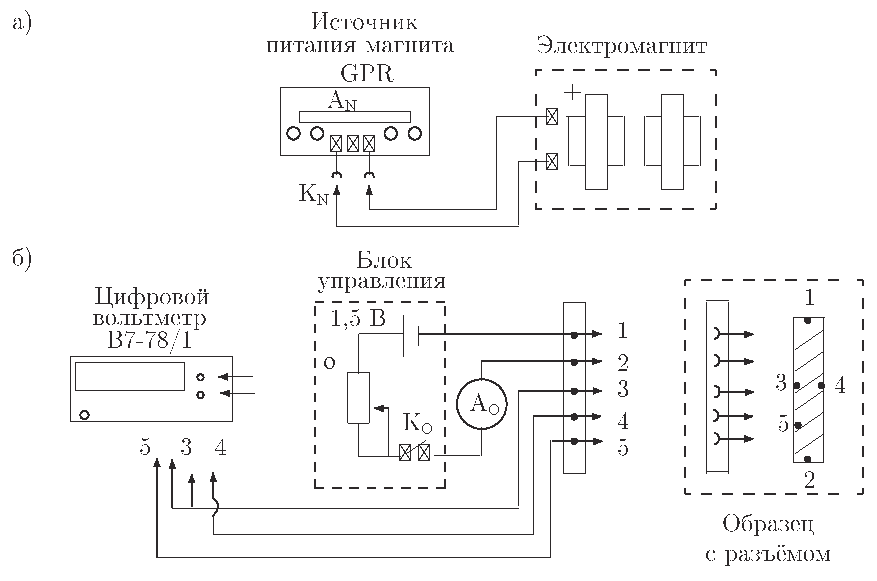
\includegraphics[scale=0.9]{ustanovka.pdf}}
		\caption{Схема установки для исследования эффекта Холла в полупроводниках.}
		\label{ris:ustanovka}
	\end{figure}
%\section{Модель эксперимента}
\newpage
\section{Экспериментальные данные}
	%В таблице~\ref{table:const} приведены константы, используемые в лабораторной работе. 	
	\floatsetup[table]{capposition=top}	
	\begin{table}[H]
		\caption{Параметры установки и исследуемого образца.}
		\label{table:const}
		\begin{tabular}{|c|c|c|c|}
			\hline
			\begin{tabular}[c]{@{}c@{}}Расстояние между\\ контактами 3 и 5\\ $L_{35}$, мм\end{tabular} & \begin{tabular}[c]{@{}c@{}}Толщина образца\\ $a$, мм\end{tabular} & \begin{tabular}[c]{@{}c@{}}Ширина образца\\ $l$, мм\end{tabular} & \begin{tabular}[c]{@{}c@{}}Постоянная катушки\\ $SN$, см$^2\cdot\,$вит.\end{tabular} \\ \hline
				6                                                                                          & 2,2                                                               & 7                                                                &                                                                 72                   \\ \hline
			\end{tabular}
	\end{table}
		
		
	%В таблице~\ref{table:error} приведены значения и случайные ошибки измерения величин, определяемых в ходе эксперимента.
	\floatsetup[table]{capposition=top}	
	\begin{table}[H]
		\caption{Некоторые измеряемые величины и их погрешность.}
		\label{table:error}
		\begin{tabular}{|c|c|c|c|c|}
			\hline
			& $\Phi$, мВб & $I_M$, А & $U_{34}$, мкВ & $I$, мА \\ \hline
			Величина          & 1,0         & 1,00     & 50          & 0,5     \\ \hline
			Погрешность       & 0,1         & 0,01     & 1           & 0,005   \\ \hline
			$\varepsilon$, \% & 1           & 1        & 2           & 1       \\ \hline
		\end{tabular}
	\end{table}


	\floatsetup[table]{capposition=top}	
	\begin{table}[H]
		\caption{Калибровка электромагнита.}
		\label{table:calibration}
		\begin{tabular}{|c|c|c|c|c|c|c|c|c|c|c|}
			\hline
			№           & 1    & 2    & 3    & 4    & 5    & 6    & 7    & 9    & 9    & 10   \\ \hline
			$I_M$, A    & 0,61 & 0,71 & 0,83 & 0,91 & 1,06 & 1,11 & 1,15 & 1,22 & 1,38 & 1,45 \\ \hline
			$\Phi$, мВб & 4,2  & 4,7  & 5,4  & 5,8  & 6,6  & 6,7  & 6,9  & 7,1  & 7,6  & 7,7  \\ \hline
			$B$, мТл    & 583  & 653  & 750  & 806  & 917  & 931  & 958  & 986  & 1056 & 1069 \\ \hline
		\end{tabular}
	\end{table}


	\floatsetup[table]{capposition=top}	
	\begin{table}[H]
		\caption{Зависимость $U_{34}$ от $I_M$ при фиксированном $I$.}
		%\footnote{Измерения проводились при калиброванных значениях магнитной индукции катушки}
		\label{table:U_34}
		\begin{tabular}{|c|c|c|c|c|c|c|c|c|c|c|}
			\hline
			$I$, мА    & 0,24 & 0,26 & 0,28 & 0,30 & 0,35 & 0,45 & 0,65 & 0,85 & 1,00 & 1,00 \\ \hline
			$U_0$, мкВ & -49  & -56  & -61  & -65  & -77  & -100 & -140 & -183 & -220 & -220 \\ \hline
			№          & \multicolumn{10}{c|}{$U_{34}$, мкВ}                                 \\ \hline
			1          & -2   & -2   & -5   & -4   & -5   & -7   & -5   & -5   & -13  & -450 \\ \hline
			2          & 4    & 4    & 4    & 3    & 4    & 4    & 10   & 15   & 10   & -480 \\ \hline
			3          & 11   & 10   & 10   & 11   & 13   & 17   & 28   & 35   & 35   & -508 \\ \hline
			4          & 16   & 15   & 17   & 17   & 21   & 26   & 41   & 55   & 58   & -533 \\ \hline
			5          & 23   & 24   & 25   & 25   & 30   & 38   & 58   & 76   & 85   & -560 \\ \hline
			6          & 25   & 25   & 27   & 28   & 33   & 44   & 65   & 84   & 94   & -570 \\ \hline
			7          & 27   & 27   & 29   & 30   & 35   & 46   & 70   & 90   & 100  & -577 \\ \hline
			8          & 28   & 29   & 30   & 33   & 39   & 50   & 74   & 97   & 110  & -587 \\ \hline
			9          & 32   & 32   & 35   & 37   & 44   & 56   & 84   & 108  & 125  & -603 \\ \hline
			10         & 34   & 35   & 38   & 40   & 47   & 60   & 89   & 115  & 132  & -613 \\ \hline
		\end{tabular}
	\end{table}

Дополнительно при силе тока в 1 мА, протекающем через образец, измерим $U_{35} = -2,531$ мВ.
		
\newpage
\section {Обработка результатов}
	Для калибровки электромагнита необходимо экстраполировать график зависимости $B = f(I)$ (рис.~\ref{ris:B=f(I)}). Не трудно убедиться, что с большой точностью зависимость является линейной в данном диапазоне токов. С меньшей достоверностью зависимость можно описать многочленом третей степени, на который хорошо ложатся экспериментальные точки. Однако в связи прецизионностью источника питания нам достаточно знать конечный набор значений магнитного поля $B$ и проводить измерения $U_{34}$ только на них.
	\begin{figure}[H]
		\center{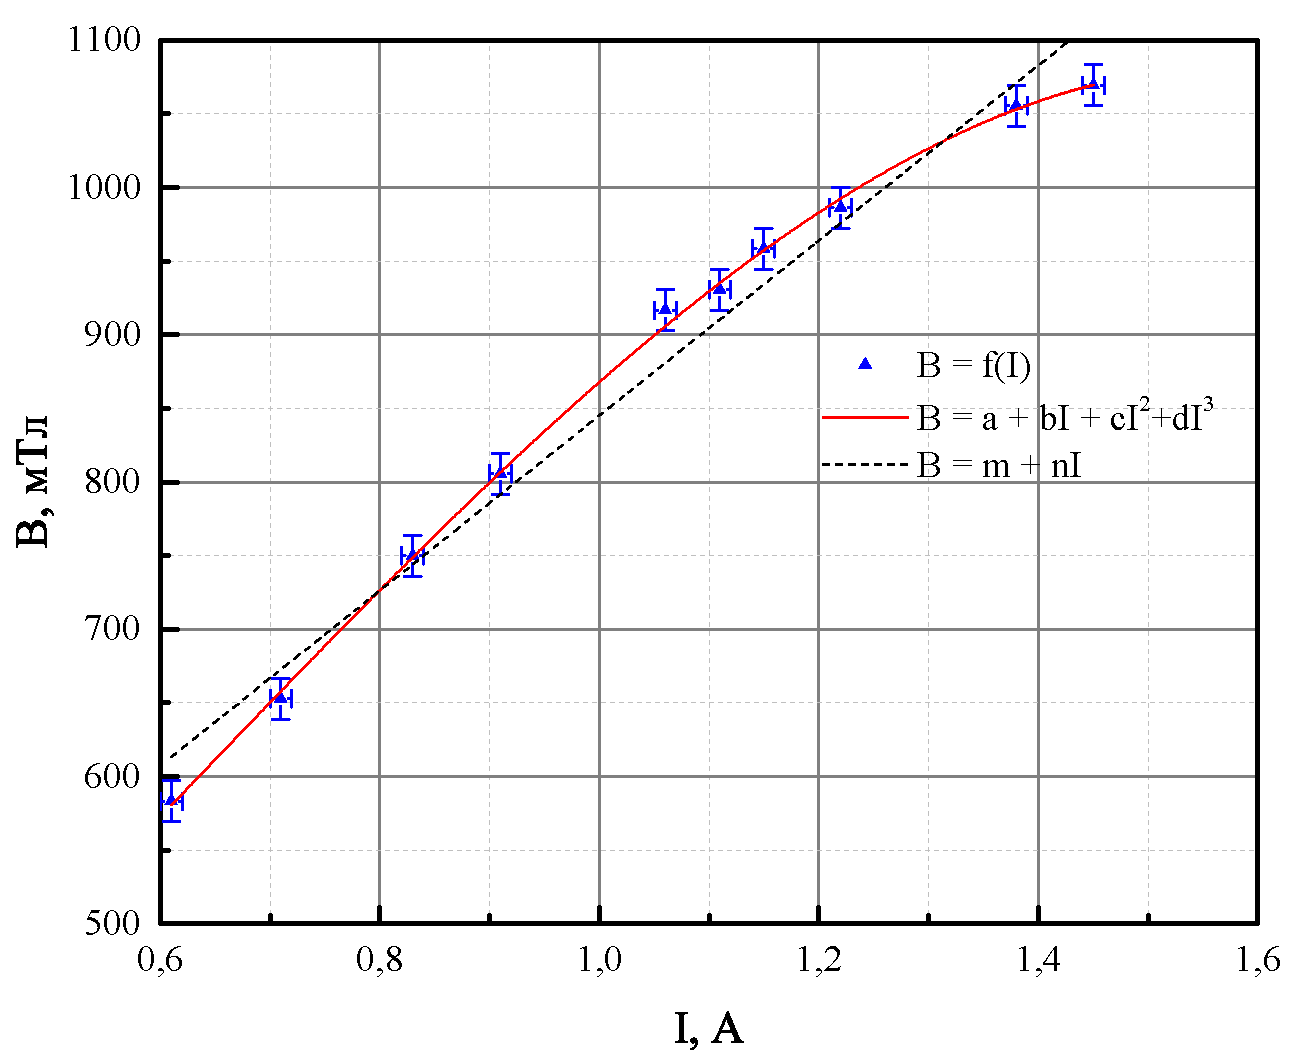
\includegraphics[scale=0.4]{B=f(I).pdf}}
		\caption{Зависимость $B = f(I)$.}
		\label{ris:B=f(I)}
	\end{figure}


	Построим серию прямых $\mathscr{E}_\text{х} =\mathscr{E}_\text{х} (B)$ (рис.~\ref{ris:Ex}). Отметим, что $\sigma_{\mathscr{E}_\text{х}} = 2 \sigma_{U_{34}} = 2$~мкВ, а $\sigma_B = \sigma_\Phi / SN = 14$ мТл.
	\begin{figure}[H]
		\center{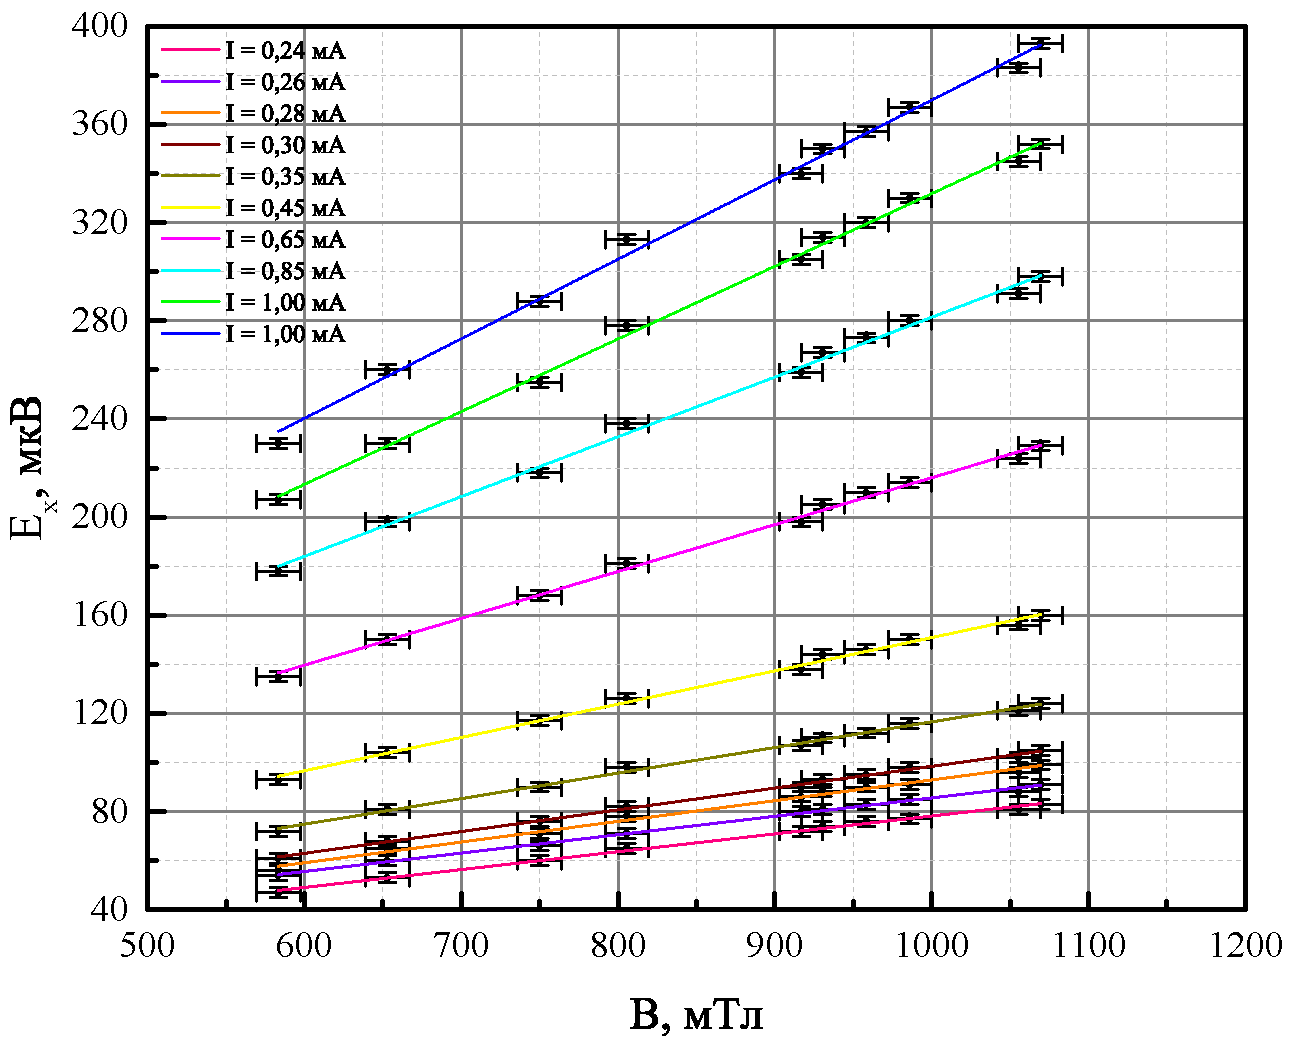
\includegraphics[scale=0.5]{Ex.pdf}}
		\caption{Серия зависимостей $\mathscr{E}_\text{х}$ от $B$ при различных $I$.}
		\label{ris:Ex}
	\end{figure}
\newpage
		\begin{table}[H]
		\caption{$k = \Delta \mathscr{E}_\text{х} / \Delta B $.}
		\label{table:k}
		\begin{tabular}{|c|c|c|c|c|c|c|c|c|c|c|}
			\hline
			$I$, мА            & 0,24 & 0,26 & 0,28 & 0,3,0 & 0,35 & 0,45 & 0,65 & 0,85 & 1,00 & 1,00 \\ \hline
			$k$, мкВ/Тл        & 72,7 & 74,9 & 84   & 88,6  & 104  & 136  & 191  & 244  & 296  & -324 \\ \hline
			$\sigma_k$, мкВ/Тл & 1,6  & 1,7  & 2    & 1,7   & 2    & 3    & 4    & 6    & 5    & 7    \\ \hline
		\end{tabular}
	\end{table}


	По полученным данным построим график зависимости $k$ от $I$ и проанализируем его.
	\begin{figure}[H]
		\center{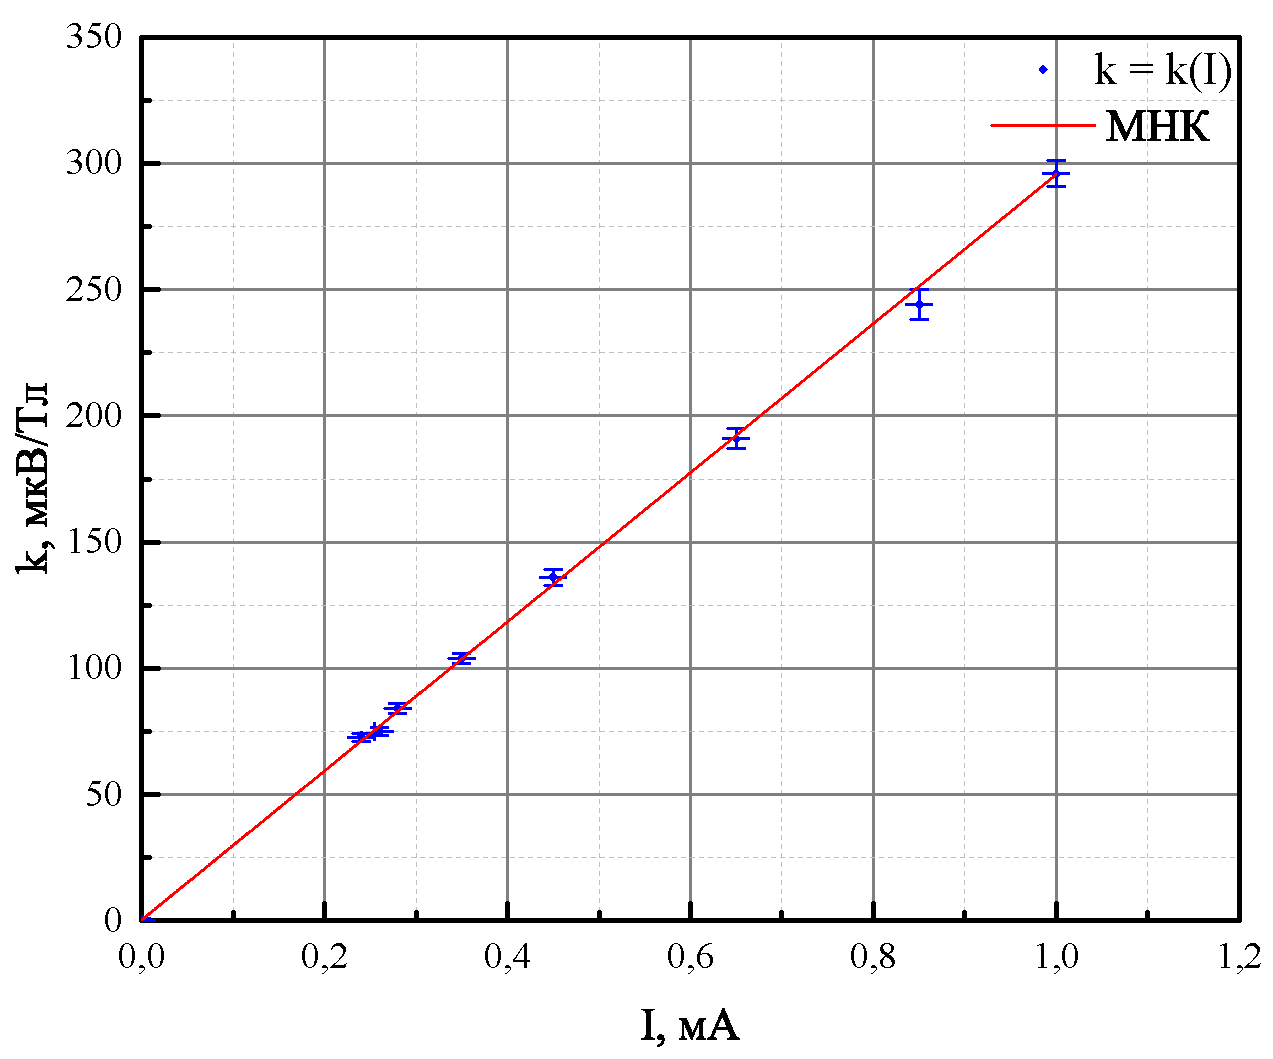
\includegraphics[scale=0.5]{k=k(I).pdf}}
		\caption{Зависимость $k$ от $I$.}
		\label{ris:k=k(I)}
	\end{figure}


	Методом наименьших квадратов определяем, что $k/I = (295\,\pm\,3)$ $\frac{\text{мВт}}{\text{Тл}\cdot\text{А}}$, откуда согласно формуле~(\ref{R}) $R_\text{х} = (649\,\pm\,7)$ см$^3$/Кл.
	
	Рассчитаем концентрацию носителей тока в образце по формуле~(\ref{n}): $n = (962\,\pm~\,1)~\cdot~10^{19}\,\text{м}^3$, удельную проводимость по формуле (\ref{sigma}): $\sigma = (153,9\,\pm\, 0,8)$ (Ом$\cdot$м)$^{-1}$.
	 
	Вычислим подвижность носителей тока в материале образца по формуле~(\ref{b}):
	 \[
	\boxed{b = (1000\,\pm\, 10) \frac{\text{см}^2}{\text{В}\cdot\text{с}}}
	\]
\section {Обсуждение результатов}
	В ходе данной лабораторной работы мы исследовали эффект Холла в полупроводнике, а именно в Германии. Нам удалось определить постоянную Холла, которая в данных диапазонах токов и значений магнитной индукции магнитного поля оказалась постоянной и равной $R_\text{х} = 649$ см$^3$/Кл с относительной ошибкой 1\%. Так же вычислили концентрацию носителей тока в образце при том предположении, что количество носителей одного типа намного больше другого типа: $n = 962\, \cdot \, 10^{19}\,\text{м}^3$. Зная направление тока в проводнике, полярность вольтметра, направление тока в катушках, можно определить тип проводимости. В нашей работе тип проводимости в Германии оказался дырочным.
	
	Более того, мы вычислили подвижность дырок в исследуемом Германии: $b = 1000\, \frac{\text{см}^2}{\text{В}\cdot\text{с}}$ с точностью в 1\%. Но наш результат отличается от табличного для носителей в области собственной проводимости $b_0 = 1800\, \frac{\text{см}^2}{\text{В}\cdot\text{с}}$ (при температуре $T$ = 293 К), по чему можно сделать вывод, что наш образец является не чистым, а с примесями. Хотелось бы отметить, что дополнительная ошибка измерений может быть связана с сильной зависимостью концентрации основных носителей токов от температуры. Действительно, для отрыва электрона от атома полупроводника и превращения его в электрон проводимости необходимо сообщить ему некоторое колличество энергии. Естественно, что такая энергия поставляется тепловыми колебаниями атомов решетки. В нашей работе температура температура образца была как минимум комнатной ($T = 298$ К) и как максимум могла повыситься вследствие протекающего через образец постоянного тока.
	
	
\section{Выводы}
	\begin{enumerate}
		\item 
			Вычислили постоянную Холла: $R_\text{х} = (649\,\pm\,7)$ см$^3$/Кл;
		\item 
			Определили концентрацию носителей тока в образце: $n = (962\,\pm~\,1)~\cdot~10^{19}\,\text{м}^3$;
		\item
			Рассчитали удельную проводимость: $\sigma = (153,9\,\pm\, 0,8)$ (Ом$\cdot$м)$^{-1}$;
		\item 	
			Германий является легированным образцом с подвижностью $b = (1000\,\pm\, 10) \frac{\text{см}^2}{\text{В}\cdot\text{с}}$;
		\item
			Тип носителей в исследуемом материале - дырочный.
	\end{enumerate}








\end{document}